%%%%%%%%%%%%%%%%%%%%%%%%%%%%%%%%%%%%%%

\documentclass[12pt]{article}
%\documentstyle[12pt,psfig,epsf]{article}

\hoffset=-15mm \voffset=-25mm \textwidth=165mm \textheight=245mm
\usepackage{graphicx}
\usepackage{amsmath}
\usepackage{amssymb}
%\usepackage{bigcircle}
\usepackage{wrapfig}
\usepackage{indentfirst}
\usepackage{color}
\usepackage{subfigure}

\begin{document}

\vskip 0.5cm \centerline{\bf\Large Vector meson production}
\centerline{\bf\Large in ultra-peripheral collisions at hadronic colliders}  \vskip 0.3cm
\centerline{R.~Fiore $^a$, L.~Jenkovszky $^{b\star}$, V.~Libov$^c$, and Magno V. T. Machado$^d$}

\vskip 1cm

\centerline{$^a$ \sl Universita' della Calabria}
\centerline{$^b$ \sl Bogolyubov Institute for Theoretical Physics,
National Academy of Sciences of Ukraine} \centerline{\sl Kiev,
03680 Ukraine} 
\centerline{$^c$ \sl Deutsches Elektronen-Synchrotron, Hamburg, Germany}
\centerline{$^d$ \sl HEP Phenomenology Group, CEP 91501-970, Porto Alegre, RS, Brazil
}
\vskip
0.1cm

\begin{abstract}\noindent
By using a two-component Pomeron model, successfully describing the HERA data on exclusive diffractive vector meson production (VMP) and deeply virtual Compton scattering (DVCS), we analyse the data on VMP in ultra-peripheral collisions at the LHC. Predictions for future experiments on the production of $J/\Psi$ and other vector mesons are presented.
\end{abstract}

\vskip 0.1cm

$
\begin{array}{ll}

^{\diamond}\mbox{{\it e-mail address:}} &
   \mbox{vladyslav.libov@desy.de} \\
^{\star}\mbox{{\it e-mail address:}} &
   \mbox{jenk@bitp.kiev.ua} \\

%^{\ast}\mbox{{\it e-mail address:}} &
 %  \mbox{?@?.?} \\

\end{array}
$

%\end{titlepage}

\section{Introduction}\label{Int}

After the closure of HERA, exclusive diffractive production of mesons in ultra-peripheral collisions of protons and nuclei became among the priorities of the present and future studies at the LHC \cite{LHCb1, LHCb2}, triggering a large number of theoretical investigations \cite{Schafer, Brazil, Ryskin, Motyka, Szczurek}. For relevant review papers see, e.g. \cite{Review}.
The first results on vector meson production, in particular of $J/\Psi$, are already published \cite{LHCb1, LHCb2}.

In our studies of vector meson production production at the LHC we concentrate on the following issues:
\begin{itemize}

\item we investigate possible changes in the energy dependence of the cross sections when moving from HERA to the LHC, in particular we are interested the change from "soft" (light vector mesons) to those heavy ($\phi,\ \ J/\Psi,\ \ \Upsilon$ {\it etc.}) mesons;

\item apart from the "standard" (familiar) photon and Pomeron exchanges, we study the
contribution from the Odderon and secondary trajectories;

\item we study possible deviation from the exponential behaviour of the $t$-dependence
(the forward cone);

\item because of the long range of the electromagnetic interactions, ultra-peripheral collisions imply real photon exchange, which is not neccesarily true for the exchnge of the Pomeron and other strongly interacting (short range) reggeons;  therefore, differently from the papers of our predecessors \cite{Schafer, Brazil, Ryskin, Motyka, Szczurek}, we consider also electroproduction ($Q^2\neq 0$).

\end{itemize}

\section{Simple parametrizations of $\sigma_{\gamma p\rightarrow Vp}(\omega)$;\\
The photon flux}\label{simple}

The vector meson production (VMP) cross section, Fig. 1, can be written in a factorized form, see \cite{Brazil, Review} 
(see, e.g. Eqs. (1) and (9) in \cite{Brazil}a)) is
The distribution in rapidity $Y$ of the production of a vector meson $V$ in the reaction $h_1+h_2\rightarrow h_1Vh_2,$ (where $h$ may be a hadron, e.g. proton, or a nucleus, pPb, PbPb,...) is calculated according to a standard prescripion base on factorization of the photon flux and photon-proton cross section (see below).

\begin{figure}[!h]
\centering
 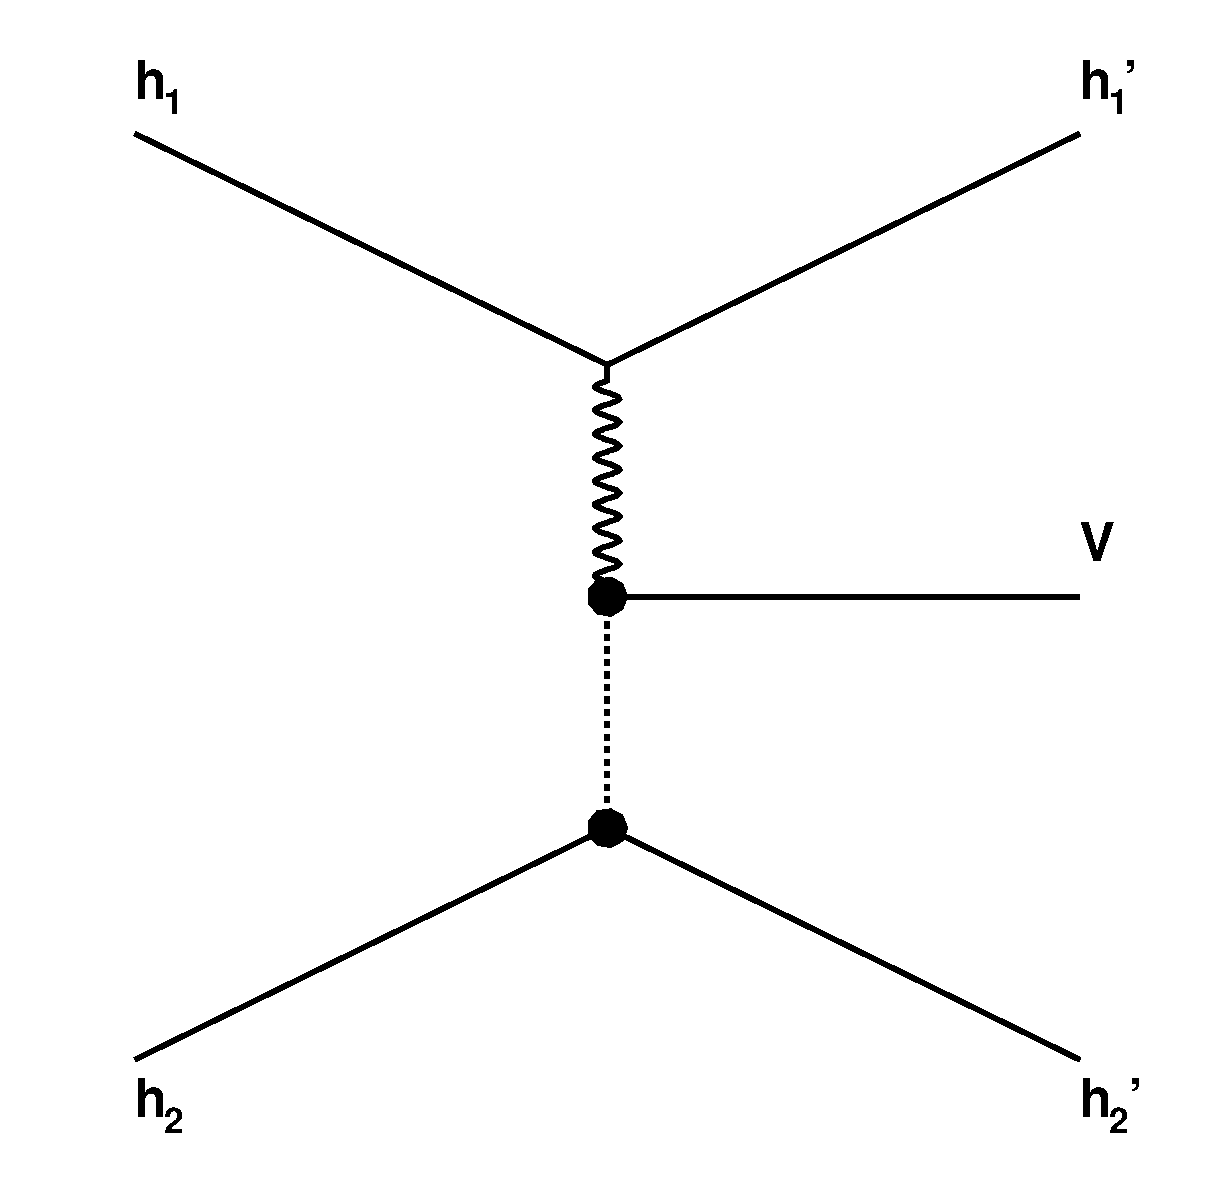
\includegraphics[width=.4\textwidth]{figures/exclusive_vmp.eps}
 \caption{Feynman diagram of vector meson production in hadronic collision.}
 \label{fig:vmp_feynman}
\end{figure}

Generally speaking, the $\gamma p$ cross section depends on three variables: the total energy of the $\gamma p$ system, $W_{\gamma p}$,
the squared momentum transfer $t$ and virtuality $\tilde Q^2=Q^2+M_V^2$, where $Q^2=-q^2$ is the photon virtuality. Since, by definition, in ultraperipheral, $b>>R_1+R_2,$
collisions, where $b$ is the impact parameter, i.e. the closest distance between the centres of the colliding particles/nuclei) and R is their radii,
photons are nearly real, $Q^2=0$, $M_V^2$ remains the only measure of "hardness". (NB: this may not be true for the peripheral $b\sim R_1+R_2$ collisions and in
Pomeron or Odderon exchange instead of the photon.) Finally, the $t$-dependence (shape of the diffraction cone) is known to be exponential. It can be either integrated, or 
kept explicit. Extending this parametrization to include a $t-$dependent exponential is easy (see below). In any case, $\sigma_{\gamma p\rightarrow Vp}(\omega)$ is well known from HERA.
{\bf(so far we haven't introduced $\omega$!)}

We start with a simple parametrization of the $\sigma_{\gamma p\rightarrow Vp}(\omega)$ cross section, $\sigma(W)=\int_{t_m}^{t_{thr}}\frac{d\sigma}{dt},$
suggested by Donnachie and Landshoff \cite{DL}: $\sigma(W)\sim W^{\delta},\ \delta\approx 0.8$ (more involved models, e.g. of Ref. \cite{Capua, Fazio}
will be considered below), and we remind that $W_{\gamma p}^2=2\omega\sqrt {s}$.

 Let us rewrite Eq. (\ref{1}) as
 \begin{equation}\label{1}
\frac{d\sigma (h_1+h_2\rightarrow h_1+V+h_2)}{dY}=\omega_+\frac{dN_{\gamma/h_1}(\omega_+)}{d\omega}\sigma_{\gamma h_2\rightarrow Vh_2}(\omega_+)+
\omega_-\frac{dN_{\gamma/h_2}(\omega_-)}{d\omega}\sigma_{\gamma h_1\rightarrow Vh_1}(\omega_-),
\end{equation}
where $\frac{dN_{\gamma/h}(\omega)}{d\omega}$ is the "equivalent" photon flux \cite{Review} 
$\frac{dN_{\gamma/h}(\omega)}{d\omega}=\frac{\alpha_{em}}{2\pi\omega}[1+(1-\frac{2\omega}{\sqrt{s}})^2]
(\ln\Omega-\frac{11}{6}+\frac{3}{\Omega}-\frac{3}{2\Omega^2}+\frac{1}{3\Omega^3})$
and $\sigma_{\gamma p\rightarrow Vp}(\omega)$ is the total (integrated in $t$) cross section of the vector meson photoproduction subprocess (same as e.g. at HERA, see \cite{Capua, Fazio}). Here $\omega$ is the photon energy, $\omega=W^2_{\gamma p}/2\sqrt s_{pp}$ with
$\omega_{min}=M_V^2/(4\gamma_Lm_p),$ where $\gamma_L=\sqrt s/(2m_p)$ 
is the Lorentz factor (Lorentz boost of a single beam), e.g., for pp at the LHC for $\sqrt{s}=7$~TeV,
$\gamma_L=3731$.
%,giving $W_{\gamma p}=960$ GeV.
Furthermore,
$\Omega=(\xi ?!)=1+Q_0^2/Q_{min}^2,\  Q_{min}^2=\omega/\gamma_L^2,\   Q_0^2=0.71GeV^2,\   x=M_Ve^{(-y)}/\sqrt s,\  Y\sim\ln(2\omega/m_V)$ is rapidity, $y=Y(?$).
 The subscripts $\pm$ should be respected following Eq. (\ref{1}).
Furthermore we have: $\Omega=1+Q^2_0/Q^2_{min}$, where $Q_0^2=0.71,\ \ Q_{min}^2=\omega/\gamma^2_L,\ \omega=m_Ve^Y/2$, hence $\Omega_i=1+0.71\gamma_L^2,\ \ \gamma_L^2=7/(2m_p)\approx 3.57, \  \
m_{V=J/\Psi}=3.1, \sqrt{s}=7, \ \alpha_{em}/(2\pi)\approx 10^{-3},$ hence $Q^2_{min}\approx 5.54e^Y,\ \ \Omega=1+3.9e^{-Y}$. For definiteness we fix: a) the colliding particles are protons;
b) the produced vector meson $V$ is $J/\Psi$, and 3) the collision energy $\sqrt s=7$ TeV.
We comprise the constants in $A=\alpha_{em}/(2\pi),\ \  c=Q_0^2\gamma_L^2$.
(Notice that the shape of the distribution in $Y$ is very sensitive to the value (and the sign) of the constant $c$!). The $i=\pm$ signs of $\omega$ correspond to the first or second term in Eq. (\ref{1}), respectively, $\omega_{\pm}\sim e^{\pm Y}$.

To fix the notation, basic parameters and show the difference in the energy ($W$) dependence of the produced vector meson, we start with a "pedagogical" example containing the standard photon flux and the simplest model for $\sigma(W)\sim W^{0.8}$, without any $t$ or $Q^2$ dependence ({\it i.e.} photoproduction for $t=0$) {\bf(is it $t$=0 or integrated over $t$??)}.
Fig.~\ref{fig:sigma_y_simple} shows the distribution in rapidity $Y$. Fig.~\ref{fig:sigma_w_simple} shows the energy dependence of $J/\Psi$ photoproduction cross section at the LHC ($\sqrt{s}=7$ TeV) (solid line)
compared with that at HERA \cite{Fazio} (dashed line) {\bf (this is pp cross section so comparison to HERA not possible!?)}.

\begin{figure}[!h]
  \centering
  \subfigure[]{\label{fig:sigma_y_simple}
    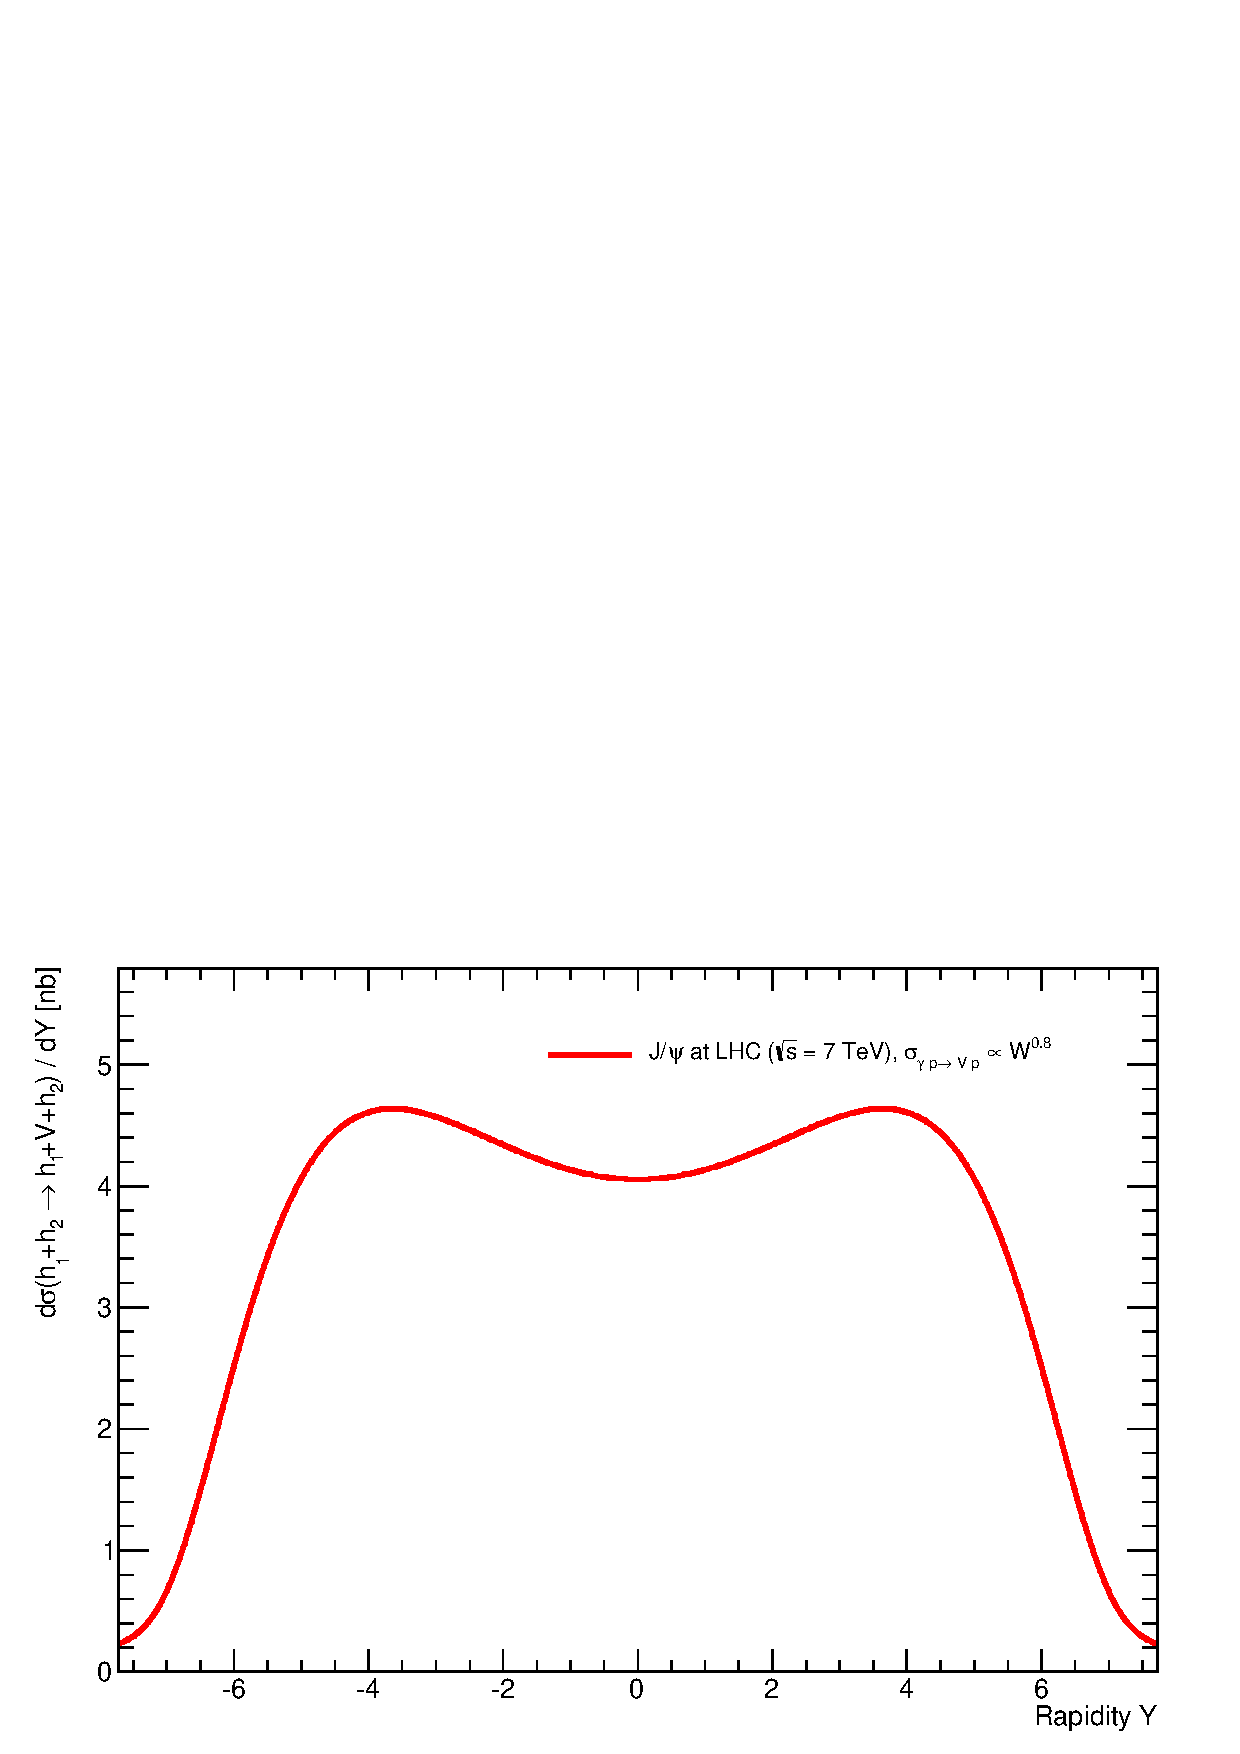
\includegraphics[height=5cm]{figures/sigma_y_simple}
  }
  \subfigure[]{\label{fig:sigma_w_simple}
    \includegraphics[height=5cm]{figures/sigma_w_simple.eps}
  }
  \caption{Differential cross section as a function of rapidity $Y$ (a) and photon-proton centre-of-mass energy (b).}
\end{figure}

In subsequent sections we extend the simple model of the previous section, namely:
\begin{itemize}
\item We include $t$ dependence - both exponential (corresopong to linear Regge trajectories) and with deviations from the exponential (from linar Regge trajectories); 
\item In the $\sigma_{\gamma p \rightarrow V p}$ cross section we include, apart from $W$ and $t$ dependence, also $Q$ dependence, negligible in $\gamma-$ but important in Reggeon (Pomeron, Odderon,...) exchanges. 
\item We include corrections due to rapidity gap survival probability.
\end{itemize} 

\section{Realistic model of $\gamma p\rightarrow V$ cross section}\label{realistic}
A simple model for $J/\Psi$ photoproduction ("testing field for diffraction"), based on a dipole Pomeron exchange 
was proposed in paper \cite{Francesco}. The model, Eqs. (5)-(7) of 
Ref. \cite{Francesco}, with a limited number (five) of adjustable parameters, fits the data on $J/\Psi$ photoproduction, and it can be used for our purposes.

Another simple and efficient model was suggested and applied to deeply virtual Compton scattering (DVCS) in Ref. \cite{Capua}. Apart from $W$ and $t$, it contains alwo dependence on virtuality $Q^2$.
The model was fitted to the HERA data on DVCS, but it can be applied also to vector meson production (VMP) by refitting its parametes.
Instead, below we shall use two versions of the so-called Reggeometric model of VMP and DVCS, suggested in Refs. \cite{Fazio}a) and \cite{Fazio}b).
Its first version \cite{Fazio} a) applies to photoproduction ($Q^2=0$), and the integrated phopoptoduction cross section, Eq. (11) in Ref. \cite{Fazio}a), is
\begin{equation}
\sigma_{el}=A_0^2\frac{(s/s_0)^{2(\alpha_0-1)}}{(1+\tilde Q^2/Q^2_0)^{2n}[2\alpha'\ln(s/s_0)+4\Bigl(\frac{a}{\tilde Q^2}+\frac{b}{2m_N^2}\Bigr)]},
\end{equation}
where $\tilde Q^2=Q^2+m_V^2$ and the parameters, fitted \cite{Fazio}a) to $J/\Psi$ photoproduction, quoted in
Table II of Ref. \cite{Fazio}a), are: $A_0=29.8\pm 2.8,\ \ Q_0^2=2.1\pm 0.4,\ \ 
n=1.37\pm 0.14,\ \ \alpha_0 =1.20\pm 0.02,\ \ \alpha'=0.17\pm 0.05, a=1.01\pm 0.11,\ \ b=0.44\pm 0.08,\ \ s_0=1$ and relevant dimensions here again are implied.
Fig.~\ref{fig:sigma_y_realistic} shows the calculated rapidity distributions for $J/\Psi$ production at the LHC while Fig.~\ref{fig:sigma_w_realistic} shows the $W$ dependence of the produced $J/\Psi$.

\begin{figure}[!h]
  \centering
  \subfigure[]{\label{fig:sigma_y_realistic}
    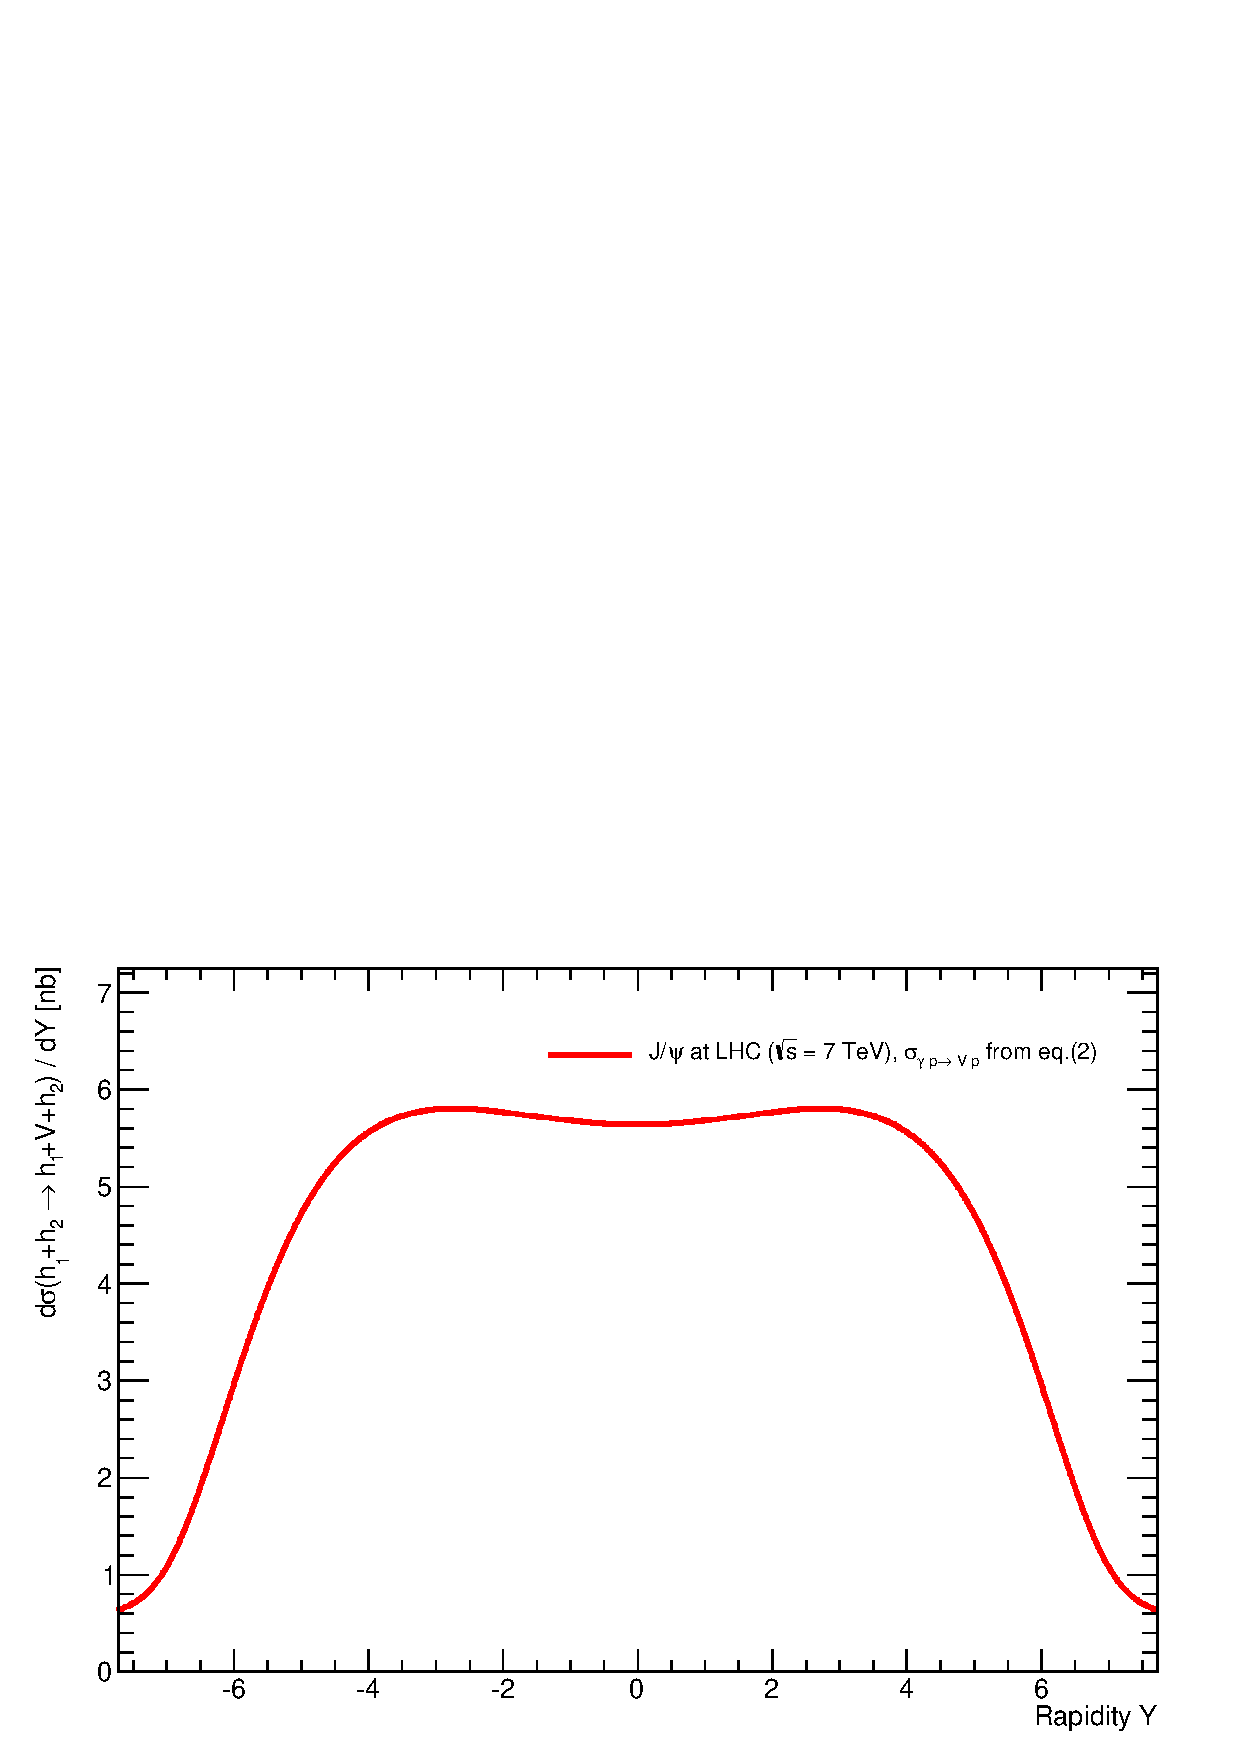
\includegraphics[height=5cm]{figures/sigma_y_realistic}
  }
  \subfigure[]{\label{fig:sigma_w_realistic}
    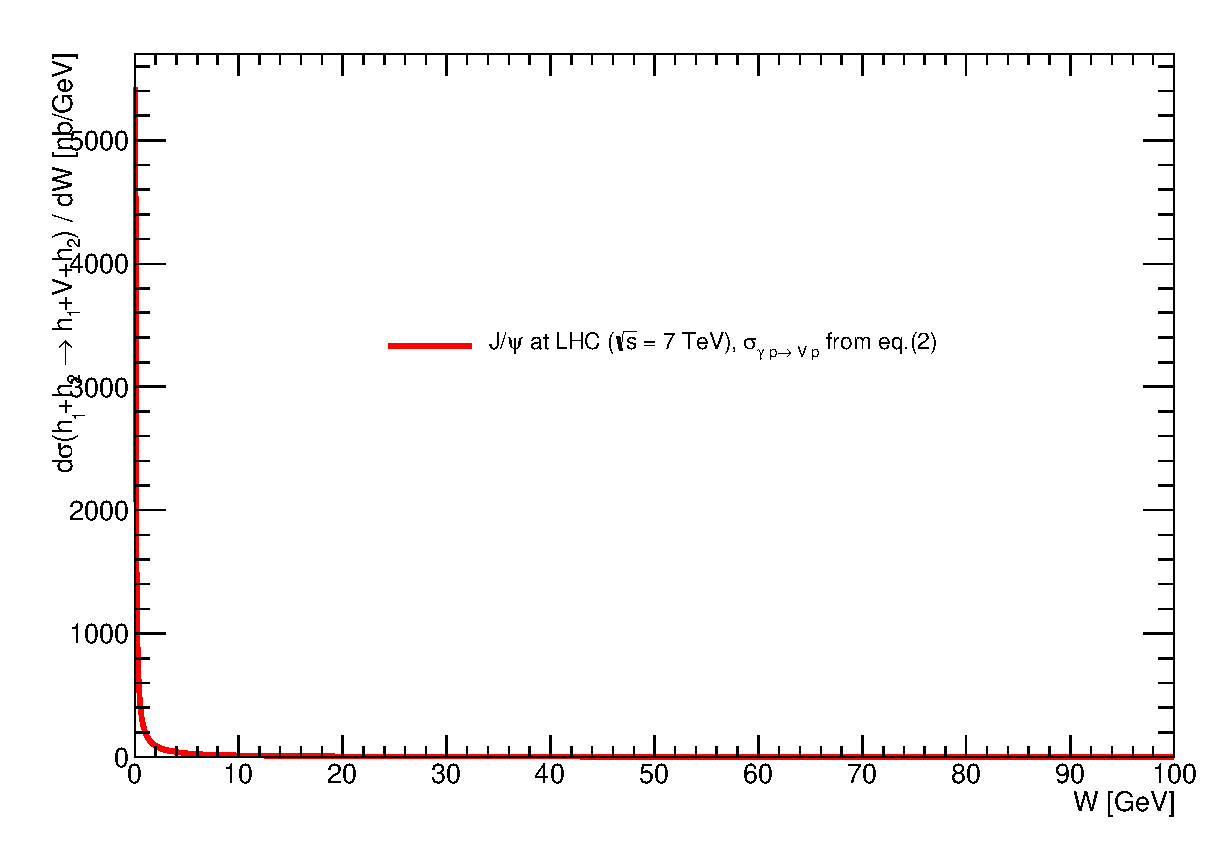
\includegraphics[height=5cm]{figures/sigma_w_realistic}
  }
  \caption{Differential cross section as a function of rapidity $Y$ (a) and photon-proton centre-of-mass energy (b).}
\end{figure}


A more advanced version of the Reggeometric model, Ref. \cite{Fazio}b) includes also $Q^2-$ dependence (electroproduction), the universal "Reggeometric" Pomeron containing two terms, a "hard" and a "soft" one, their relative weight depending on $\tilde Q^2$. Te relevant scattering amplitude is quoted in Eq. (13) of Ref. \cite{Fazio}b) with the fitted parameters collected in Tables 2 to 4 of of the same paper.

The calculated cross sections together with the new data from Refs. \cite{LHCb1, LHCb2} are shown in Figs. ......

\section{Corrections for rapidity gap survival probabilities}\label{corrections}
The above results may be modified by initial and final state interactions,
alternatively called as rescattering corrections. The calculation of these
corrections is by far not unambiguous, the result depending both on the input 
and on the unitarization procedure chosen. The better (more realistic) the input, the smaller the unitarity (rapidity gap survival probability) corrections. 
Since this is a complicated and controversial issue {\it per se} deserving special studies beyond the scope of the present paper, to be coherent with the "common trend", here we use only familiar results from the literature. The standard prescription is to multiply the scattering amplitude (cross section) by a factor (smaller than one), depending on energy and eventually other kinematical variables. 
We borrow the values of these correction factors from Ref.\cite{Ryskin} b), calculated accorging to Eq.(18) and collected in Table 2, both in that paper.

The obtained (corrected) results are shown in Fig... and are compared with the results of our calulations in Sec.\ref{realistic}.

\section{Pomeron, Odderon and other($\omega, {\it f},...$) Reggeon exchanges}\label{Reggeons}

\section{Inelastic photoproduction} 
In this section we study inelastic VMP, where a small number of additional particles are produced due to either gluon radiation and/or (c,d) proton dissociation, see Fig.~\ref{fig:vmp_non_exlcusive}.

\begin{figure}[!h]
\centering
 \includegraphics[width=.8\textwidth]{figures/non_exclusive_jpsi}
 \caption{Feynman diagrams of non-exclusive $J\psi$ meson production.}
 \label{fig:vmp_non_exlcusive}
\end{figure}

\section{Conclusions}

\section*{Acknowledgements}
%\small

\begin{thebibliography}{99}
\bibitem{LHCb1} LHCb Collab., R. Aaji {\it et al., Exclusive ...}, J. Phys. {\bf G40} (2013) 045001, arXiv:1301.7084.

\bibitem{LHCb2}  LHCb Collab., R. Aaji {\it et al., Updated ...}, arXiv:1401.3288. 

\bibitem{Schafer} A. Sch\"afer, L. Mankiewicz and O. Nachtmann, Phys. Lett. {\bf B272} (1991) 419.

\bibitem{Review} G. Baur {\it et al.} Phys. Rept. {\bf 364} (2002) 359, arXiv: hep-ph/011221; K. Hencken {\it et al.}, in: Phys. Rept. {\bf 458} (2008) 1.

\bibitem{Brazil} a) V.P. Goncalves and M.M. Machado, {\it Heavy quark production...}, arXiv: 1112.3500;
b) V.P. Goncalves and M.M. Machado, {\it Quarkonium+...}, arXiv: 1207.5273 [hep-ph]; c) V.P. Gonsalves and W.K. Suter, arXiv: 1004.1952 [hep-ph];
d) V.P. Goncalves and M.M. Machado, {\it Vector meson production...}, arXiv: 1106.3036 [hep-ph]; e) V.P. Goncalves, {\it Probing the Odderon...},
arXiv: 1211.1207 [hep-ph]; f) M.B. Gay Ducati, M.T. Griep and M.V.T. Machado, {\it Exclusive photoproduction of...}, arXiv: 1305.4611 [hep-ph]; 
g) V.P. Goncalves and M.M. Machado, {\it Photoproduction of ...}, arXiv: 0907.4123 [hep-ph].

\bibitem{Ryskin} a) V.A. Khoze, A.D. Martin, and M.G. Ryskin, {\it Photon-exchange...}, arXiv: 0201301 [hep-ph]; 
b) S.P. Jones, A.D. Martin, and M.G. Ryskin and T. Teubner, {\it Probes of...} arXiv:1307.7099 [hep-ph]; 
c) S.P. Jones, A.D. Martin, and M.G. Ryskin and T. Teubner, {\it Predictions of...} arXiv: 1312.6795 [hep-ph].

\bibitem{Motyka} a) A. Bzdak {\it et al., Exclusive...}, arXive:hep/ph/0702134; b) L. Motyka and G. Watt, {\it Exclusive...}, arXiv:0805.2113.  

\bibitem{Szczurek} a) W. Sch\"afer and A. Szczurek, {\it Exclusive...}, arXiv:0705.2887 [hep-ph]; b) W. Sch\"afer, G. Slipek and A. Szczurek,
{\it Exclusive...} Phys. Letters {\bf B688} (2010) 185. 

\bibitem{DL} A. Donnachie and P. Landshoff, Phys. Lett. {\bf B296} (1992) 227.

\bibitem{Francesco} R. Fiore, L.L. Jenkovszky, F. Paccanoni, EPJ {\bf C10} (1999) 461; arXiv hep-ph/9812458.

\bibitem{Capua} M. Capua {\it et al.}, Phys, Lett. {B645} (1997) 161; hep-ph/0605319

\bibitem{Fazio} a) S. Fazio, R. Fiore, L. Jenkovszky, A. Salii, Acta Phys. Polonica B {\bf 44} (2013) N6, 1333; b) S. Fazio, R. Fiore, L. Jenkovszky, A. Salii, 
hep-ph/1312.5683, Dec. 2013. 

\end{thebibliography}

\end{document}
